\documentclass[oribibl]{llncs}
\usepackage{llncsdoc}
\usepackage{multirow}
\usepackage{graphicx}
\graphicspath{{pics/}}
\usepackage[numbers,sort]{natbib}
\usepackage{amsmath}

\renewcommand{\refname}{References}  % for the article class
\renewcommand{\bibname}{References}  % for the report or book class

\begin{document}

\title{Searching Higher Order Mutants For Software Improvement}

\author{Author(s)
%Fan Wu\inst{1}         \and
%		Mark Harman\inst{1}        \and
%		Yue Jia\inst{1}         \and
%		Jens Krinke\inst{1}
}


\institute{Institution(s) hidden for anonymity
%Department of Computer Science, UCL, Gower Street, London WC1E 6BT, UK \\
%              \email{\{fan.wu.12,mark.harman,yue.jia,j.krinke\}@ucl.ac.uk} 
}

\maketitle

\begin{abstract}
We propose using Higher Order Mutation for Genetic Improvement of software in this paper, where the optimisation granularity is smaller than previous works but the scalability remains.
We use mutation tools to operate on the subjects in a fine granularity.
Higher Order Mutants are searched for to improve the quality of the subjects, while regression tests are used to maintain the functionality.
A prior sensitivity analysis suggests that **\% improvement on time and **\% on memory are found in First Order Mutants.
By combining First Order Mutants, we find **\% and **\% improvement on time and memory performance respectively.
A further static analysis suggests that, **\% of the mutational changes can not be achieved by previous patch-based approaches.
%\keywords{Genetic Improvement \and SBSE \and Higher Order Mutation}
\end{abstract}

\section{Introduction}
\label{sec_intro}

Optimising software for better performance such as speed and memory consumption can be demanded, especially when the resources in the running environment is limited.
Manually optimising the performance while keeping or even improving the functional behaviour of a software is challenging, 
and is even harder if the considered properties are competing with each other~\cite{Harman:2012:GCC:2351676.2351678}.
Search-Based Software Engineering (SBSE)~\cite{Harman2001833} consider this optimisation problem as a search problem, thus it can be solved by search algorithms.

Previous studies have applied different search-based techniques to automate the optimisation process~\cite{arcuri-ssbse-2011, 6035728,Brake:2008:ADS:1370018.1370031,hutter2009paramils}, however, scalability of the optimisation approaches remains as a challenge.
Recent studies use patch-based Genetic Programming to scale to large systems, where the solutions were represented as a list of patches to the subject program instead of the program itself~\cite{Bruce:2015:REC:2739480.2754752,geneticimprovementJP}.
Each patch can be inserting, deleting a piece of code, or swapping pieces of code etc..
To ensure scalability, patch-based approaches are usually line-based, therefore they are not able to fine tune the subject program in a smaller granularity. 
Wu et al. used Deep Parameter to fine tune programs, where some internal variables were exposed and optimised, with a prior sensitivity analysis on the subject programs that ensures the approach is able to scale~\cite{Wu:2015:DPO:2739480.2754648}.
However the approach follows a complicated process where redundancy may reside in the search space.

Mutation Testing~\cite{demillo1978hints,5487526} is a method to measure the quality of test cases by inserting artificial faults in the programs under test.
The programs after being inserted faults are called mutants, where mutants with a single fault are First Order Mutants (FOM) and Higher Order Mutants (HOM) are combinations of FOMs~\cite{Harman:2011:SHO:2025113.2025144}.
Despite originally used in Mutation Testing, mutants are also used in bug fixing~\cite{6035728} or sensitivity analysis~\cite{Wu:2015:DPO:2739480.2754648} due to the fact that some changes do not break the functionality of the original program, in which case the mutants are called equivalent to the original~\cite{weimerGPEM14}.

In this paper, we aim to search for Higher Order Mutants that improve the runtime performance but still preserve the functionality of the programs under optimisation~\cite{Jia:2015:GIU:2739482.2768417}.
To reduce the search space, we analyse the First Order Mutants to find the most sensitive code in the subject programs.
A following Genetic Algorithm is then applied to search for combinations of FOMs that have better runtime performance, but only mutate the most sensitive part of the programs.
We also conduct a static analysis to show how many of the changes in the optimised HOMs can not be achieved by patch-based approaches.

In this paper, we focus on two aspects of software runtime performance, execution time and memory consumption.
Time and space are important qualities for many software, especially on portable devices or embedded systems where the runtime resources are limited.
Moreover, these two qualities are usually competing with each other, yielding an interesting multi-objective solution space.
Our approach aims to search for a set of solutions, instead of one, which are not dominated by any other solutions in terms of the objectives under consideration (thus forming a Pareto front).
We evaluate our approach using four open source benchmarks with varying sizes. 
Since the approach does not require any knowledge about the subjects, it can be easily adapted to other programs.

The paper presents evidence that using Higher Order Mutation is an effective, easy to adopt way to improve existing programs. 
The experimental results suggest that equivalent FOMs can improve the subject programs by **\% on execution time or **\% on memory consumption.
Further results show that by searching for HOMs, we can achieve up to **\% time reduction or **\% memory reduction on extreme cases.
Our static analysis suggest that **\% of the changes in optimised HOMs can not be achieved by patch-based approaches.
The contributions of the paper are as follows:
\begin{enumerate}
\item We introduce an automatic searching process to improve subject programs via Higher Order Mutation, which is easy to adapt to other programs with different sizes.
\item We evaluate our approach on four open source programs with varying sizes. We report the results and demonstrate that our approach is able to reduce the execution time by up to **\% or to save the memory consumption by up to **\%.
\item The results of a static analysis are reported to show that our approach works on a smaller granularity such that **\% of the changes found by our approach can not be achieved by patch-based approaches.
\end{enumerate}

The rest of the paper is organised as follows. 
Section~\ref{sec_method} elaborates the approach we used in this paper.
Section~\ref{sec_exp} gives details on the experimental settings.
The results are reported in Section~\ref{sec_result}, followed by the discussion of threats to validity in Section~\ref{sec_threat}.
Related works are summarised in Section~\ref{sec_related}, and we conclude in Section~\ref{sec_conclusion}.

\section{Method}
\label{sec_method}

Our approach can be divided into two steps: sensitivity analysis and searching for Higher Order Mutants.
The whole process is illustrated in \figurename~\ref{fig_framework}.
The approach takes the subject under optimisation, it's test cases and the properties of interest as inputs.
It first uses a mutation engine to generate First Order Mutants of the subject program, then evaluates them to collect sensitivity information.
This process is detailed in Section~\ref{sec_sensitivity}.
In the second step, it uses FOMs and sensitivity information to search for HOMs that have better time or memory performance than the original subject.
The searching process is elaborated in Section~\ref{sec_hom}.
We ask four Research Questions in Section~\ref{sec_rq}.

\begin{figure}[h]
\centering
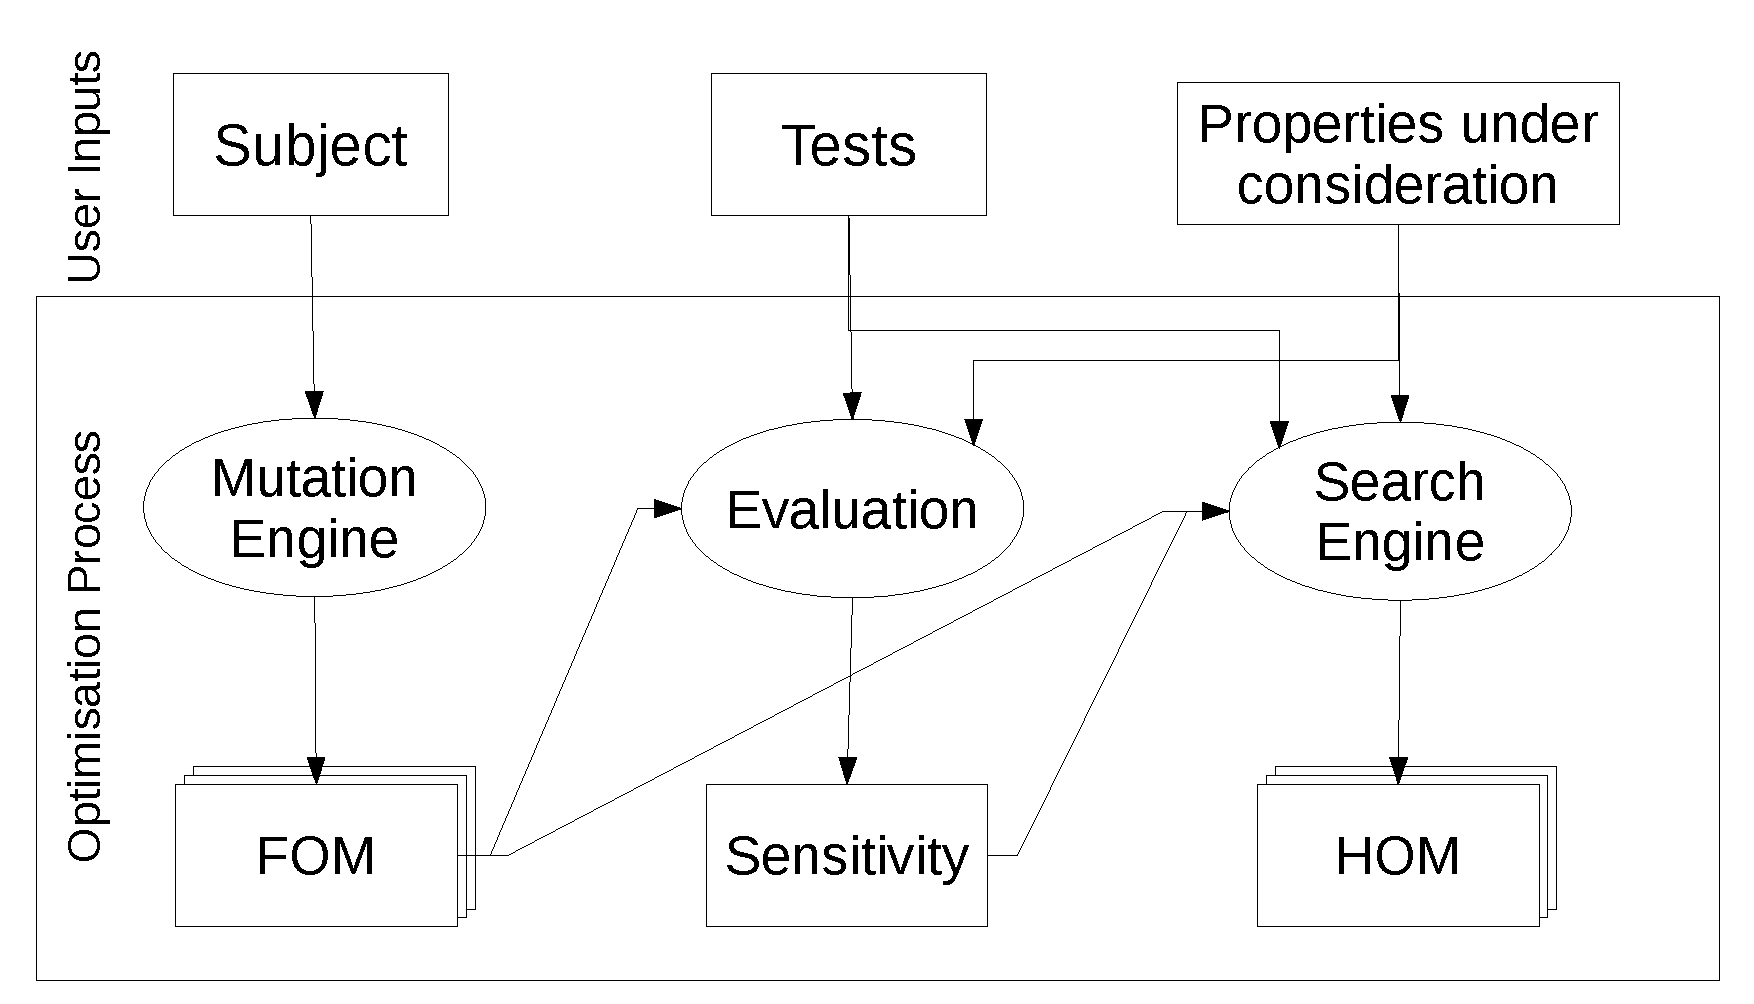
\includegraphics[width=0.7\textwidth]{framework}
\caption{Framework of Higher Order Mutants searching. Given a subject under optimisation, it's tests and the runtime properties of interest, the optimisation process first conducts sensitivity analysis on FOMs, then use this information to search for HOMs with better performance.}\label{fig_framework}
\end{figure}

\subsection{Sensitivity Analysis}
\label{sec_sensitivity}

Sensitivity analysis has been shown to be an effective way to reduce the search space in previous works~\cite{6733370,Bruce:2015:REC:2739480.2754752,6035728}.
Given a subject program under optimisation, some of the code pieces may have greater impact on the properties of interest than others.
Sensitivity analysis is to find out a small portion of the code that has the greatest impact on the properties of interest, thus the following optimisation can focus on a manageable amount of code, effectively reducing the search space.

In this paper, we use First Order Mutants to gather sensitivity information, as it was used in Wu's work~\cite{Wu:2015:DPO:2739480.2754648}.
First Order Mutants were originally used for Mutation Testing~\cite{demillo1978hints}, a method of measuring the quality of test cases by inserting artificial faults.
In Mutation Testing, a set of Mutation Operators are defined to mutate the subject program, each of which consists of a simple syntactic rule to change the subject program to generate mutants, such as changing the arithmetic operator `\texttt{+}' to `\texttt{-}'.
Mutants generated from applying a Mutation Operator once to the original program are called First Order Mutants, while those generated from applying a Mutation Operator to a mutant are called Higher Order Mutants.
We use FOMs for the sensitivity analysis because they by definition only differ from the original program in a syntactic change, therefore we can measure the sensitivity in a fine granularity.

To ensure the changes do not break the functionality, we use a regression test suite to run the mutants on.
A mutant is said to be `equivalent' with respect to a regression test suite if it passes all the regression tests.
We discard all the mutants that are not equivalent to the original since we want to preserve the correctness of the subject, then gather the runtime performance of each equivalent mutant, that is time and memory consumption in this work.
We adopt non-dominating sorting~\cite{996017} to rank all the equivalent mutants by their runtime performance, since there are two objectives under consideration.
Therefore, a code piece is said to be more sensitive than another piece if there is a FOM mutated from the first piece that is better than the best FOM mutated from the second piece in terms of their non-dominating sorting.
The range of a code piece can be defined in different ways accordingly, such as a syntactic symbol, a statement, or a nesting code block.
To avoid overlapping code pieces (meaning redundant search space), we define our code piece as a mutable symbol, which is a syntactic symbol that a Mutation Operator can be applied on.
For instance, arithmetic operator `\texttt{+}' is a mutable symbol since it can be mutated to other arithmetic operators.
After collecting the sensitivity information of all the code pieces, we feed this information to the search engine so that more sensitive code piece is more likely to be selected to form HOMs.

\begin{table}[ht]
\caption{Mutation Operators}
\label{tab_mutationoperator}
\begin{center}
\begin{tabular}{lll}
Category & Name    & Description                                          \\
\hline
\multirow{6}{*}{\begin{tabular}[c]{@{}l@{}}Selective\\ Mutation\\ Operators\end{tabular}} & ABS     & Change an expression \texttt{expr} to \texttt{ABS(expr)} or \texttt{-ABS(expr)} \\
& OAAN    & Change between \texttt{+}, \texttt{-}, \texttt{*}, \texttt{/}, \texttt{\%} \\
& OLLN    & Change between \texttt{\&\&}, \texttt{||} \\
& ORRN    & Change between \texttt{>}, \texttt{>=}, \texttt{<}, \texttt{<=}, \texttt{==} \\
& OIDO    & Change between \texttt{++}x, \texttt{{-}-}x, x\texttt{++}, x\texttt{{-}-} \\
& CRCR    & Change a constant \texttt{c} to \texttt{0}, \texttt{1}, \texttt{-1}, \texttt{c+1}, \texttt{c-1}, \texttt{c*2}, \texttt{c/2} \\
\hline
\multirow{9}{*}{\begin{tabular}[c]{@{}l@{}}Memory\\ Mutation\\ Operators\end{tabular}}    & REC2M   & Replace \texttt{malloc()} with \texttt{calloc()} \\
& RMNA    & Remove \texttt{NULL} assignment \\
& REDAWN  & Replace memory allocation calls to \texttt{NULL} \\
& REDAWZ  & Replace allocation size with \texttt{0} \\
& RESOTPE & Replace \texttt{sizeof(T)} with \texttt{sizeof(*T)} \\
& REMSOTP & Replace \texttt{sizeof(*T)} with \texttt{sizeof(T)} \\
& REM2A   & Replace \texttt{malloc()} with \texttt{alloca()} \\
& REC2A   & Replace \texttt{calloc()} with \texttt{alloca()} \\
& RMFS    & Remove \texttt{free()} statement \\
\hline
\end{tabular}
\end{center}
\end{table}

\tablename~\ref{tab_mutationoperator} lists the Mutation Operators we used in this work and their brief descriptions.
They are divided into two groups: traditional Selective Mutation Operators and Memory Mutation Operators.
We choose Selective Mutation Operators because they have been widely used in most of recent mutation analysis experiments and they have been shown their high efficiency in covering most kinds of code changes~\cite{5487526}.
Since we focus on both time and memory performance, more time/memory related Mutation Operators may provide additional potential of improvement.
Therefore we include Memory Mutation Operators~\cite{7107449,Wu2016} that mainly mutate memory management calls, which have been shown to have great impact on both time and memory performance~\cite{Zorn:1992:EMS:142181.142200}.

\subsection{Searching for Higher Order Mutants}
\label{sec_hom}

After First Order Mutants are evaluated, some equivalent mutants may be found to perform better than the original program on time and/or memory consumption.
Therefore, combining these FOMs may generate HOMs that inherit the strengths of the FOMs that they are generated from, and yield better performance than any FOM alone.
Selecting FOMs to form HOMs is a multi-objective search problem, thus we apply NSGA-II~\cite{996017} to search for HOMs with better performance.

We use an integer vector to represent a candidate HOM.
Each integer encodes whether a mutable symbol is mutated and how it is mutated.
For example, for arithmetic operator `\texttt{+}', a negative integer means it is not mutated and integer $0$, $1$, $2$, $3$ indicate that it is mutated to `\texttt{-}', `\texttt{*}', `\texttt{/}', `\texttt{\%}' respectively.
Specially, if a vector representation has only negative integers, it represents the original program, and it is an FOM if it has none but one non-negative integer.
In this representation, each vector maps to a unique HOM and all possible HOM has a unique vector representation.
Using the sensitivity information we collected earlier, we can focus on the most sensitive mutable symbols during the search algorithm.

The fitness function is as straightforward as the execution time and memory consumption over a test suite.
More formally, for each mutant $M$, the fitness of $M$ is formulated as:
$$f(M)=
\begin{cases}
    (\sum t_i(M), \sum m_i(M))       & \quad \text{if } M \text{ passes all test cases}\\
    (T_{MAX}, M_{MAX})  & \quad \text{if } M \text{ fails any test case}\\
\end{cases}
$$
where $t_i(M)$ is the time consumption of $M$ on the $i$th test case, and $m_i(M)$ is the high-water mark of the virtual memory consumption.
If $M$ fails any test case, we consider it as a bad candidate and assign it with the worst fitness values.
We choose virtual instead of physical memory consumption to measure because the physical memory consumption is not deterministic but depends on the workload of the machine, and because the virtual memory is an upper bound of the physical memory actually used.

During the search process, we maintain a population of candidate HOMs.
For each generation, crossover and mutation are performed on HOMs, generating new HOMs that are later evaluated using the fitness function above.
Tournament selection is then performed to form the next generation.
This process is repeated until a certain stopping criterion is met.
By the end of the process, the search algorithm will generate a set of non-dominating HOMs that perform better than the original program on time and/or memory consumption.

\subsection{Research Questions}
\label{sec_rq}

In this paper, we are interested in the following Research Questions.

\begin{enumerate}
\item[\textbf{RQ1}] Can First Order Mutants improve performance while maintaining functionality?
\end{enumerate}

We ask the first question as the baseline and motivation of this work.
If we find that some First Order Mutants alone have better performance than the original program, it would be interesting to search for combinations of FOMs that inherit the strengths of the FOMs.
On the other hand, if there is no FOM that outperforms the original, it would still be interesting to see whether there is synergy between FOMs such that they form HOMs that performs better than any of the FOMs alone and the original.
We answer this question by generating and evaluating FOMs, and comparing their runtime performance with the original programs.

\begin{enumerate}
\item[\textbf{RQ2}] How much improvement can be found in Higher Order Mutants, comparing with the original and FOMs?
\begin{enumerate}
\item[\textbf{RQ2.1}] How much improvement can be achieved by using traditional Mutation Operators alone?
\item[\textbf{RQ2.2}] How much improvement is accounted for by adding Memory Mutation Operators?
\end{enumerate}
\end{enumerate}

After evaluating FOMs, we are interested in searching for better performance in Higher Order Mutants.
By applying search algorithms, we expect some HOMs that inherit some or all of the strengths from the FOMs they are formed from.
We ask the second research question to understand the optimal performance we can achieve by combining FOMs.
Furthermore, it is interesting to see whether the Memory Mutation Operators help improving the performance.
Therefore, we ask two sub-questions to understand how much improvement can be achieved by using traditional Mutation Operators alone, and how much additional improvement can be achieved by adding Memory Mutation Operators.
We answer these questions by applying search algorithm on traditional mutants alone, and on traditional mutants and memory mutants together, to see the improvement respectively.

\begin{enumerate}
\item[\textbf{RQ3}] How many of the changes in improved HOMs can not be achieved by patch-based approaches?
\end{enumerate}

We ask the third research question because we want to understand whether increasing the granularity of code changes provides more improvement potential.
If there are mutational changes that can not be achieved by patching, then it is likely that some improvement may never be found by patch-based approaches, thus increasing the granularity helps in finding better performance.
We answer this question by conducting a static analysis on the source code of the subjects to see whether the mutational changes can be generated from other code pieces in the program.

\begin{enumerate}
\item[\textbf{RQ4}] Do Deep-Parameter-optimised library provide further improvement?
\end{enumerate}

Deep Parameter Optimisation is a similar work that optimises the library code instead of the source code of the subjects~\cite{Wu:2015:DPO:2739480.2754648}.
It also focused on the time and memory performance of the subjects.
Therefore it is interesting to see how the improvement changes when we link HOM-optimised subjects with Deep-Parameter-optimised libraries.
We answer this research question by evaluating the optimised HOMs after linking them to Deep-Parameter-optimised libraries, then comparing the them with their performance before the linking, and with the performance of the original program after linking to Deep-Parameter-optimised libraries.

\section{Experimental Settings}
\label{sec_exp}

In this section, we provide more details regarding the experimental settings.
The Mutation tool and the summary of the subject programs can be found in Section~\ref{sec_milu} and Section~\ref{sec_subject} respectively.
Section~\ref{sec_preprocessing} describes some techniques used to reduce the search space.
Other experimental settings can be found in Section~\ref{sec_searchsetting}.

\subsection{Milu: Mutation Engine}
\label{sec_milu}

Milu, Mutation Testing tool for C programs, is used in this work to generate mutants.
We choose Milu because it is an easy to use open source mutation tool, more importantly, it supports Higher Order Mutation, which is used in our searching process.
In order to apply Memory Mutation Operators in addition to traditional Mutation Operators consistently in the searching process, we extended the original version of Milu and implemented the Memory Mutation Operators proposed by Nanavati et al.~\cite{7107449}.
Whenever Milu is needed to generate a mutant, we transform the integer vector representation of the candidate HOM to the data format recognisable by Milu, then invoke our extended Milu to generate the HOM.

\subsection{Subjects}
\label{sec_subject}

Four subjects are used in our proof-of-concept experiments. 
\tablename~\ref{tab_subject} lists the subjects and their brief description.

\begin{table}[ht]
\centering
\caption{Subject programs}
\label{tab_subject}
%\resizebox{0.5\textwidth}{!}{
\begin{tabular}{crrl}
\hline
Name & LoC & Number of Tests & Description \\
\hline
espresso & 13256 & 19 & Digital circuit simplification\\
%\hline
gawk & 45241 & 334 & String processing\\
%\hline
flex & 9597 & 62 & Fast lexical analyzer generator\\
%\hline
sed & 5720 & 362 & Special file editor\\
\hline
\end{tabular}%}
\end{table}

\emph{Espresso} is a fast application for simplifying complex digital electronic gate circuits.
\emph{Gawk} is the GNU \emph{awk} implementation for string processing.
\emph{Flex} is a tool for generating scanners, programs which recognises lexical patterns in text, and \emph{sed} is an editor that automatically modifies files given a set of rules. 
We use the \emph{espresso} version as well as its test cases from \emph{DieHard} project~\cite{Berger:2006:DPM:1133981.1134000}.
Version 4.1.0 of \emph{gawk} is used in this work.
The source code and the test cases can be found in the GNU archives.
We obtain the last two programs and corresponding test suites from the SIR repository~\cite{SIR2005}. 

\subsection{Preprocessing}
\label{sec_preprocessing}

In order to minimise the computation in the experiments, preprocessing is conducted before each of the two steps of the experiments.
Before any FOM is generated, we first analyse the function coverage of each subject using the GNU application \emph{Gcov}.
We only mutate the functions that have non-zero coverage, since a zero-coverage function is never executed, therefore mutating it will never affect the subject program.

After collecting sensitivity information, there could be thousands of mutable locations in a subject, yielding an extremely large solution space.
Therefore we pick the first 10\% of most sensitive locations and only search for HOMs generated from mutating them, in which case spaces needed to store the vector representations of HOMs are reduced, as well as the search space.
We use a relative ratio instead of an absolute number to pick sensitive locations so that the search space is fairly adapted to the size of the subject, and 10\% is based on the observation that the locations in the first 10\% or less are usually much more sensitive than the rest of the locations.
However, the ratio can be easily adapted accordingly.

\subsection{Search Settings}
\label{sec_searchsetting}

In the experiments, NSGA-II~\cite{996017} is used to search for HOMs.
Tournament selection of size 2 and uniform crossover with probability of 0.8 are perform in each generation.
There are 50 HOMs in each generation and the algorithm stops at 100th generation.
These numbers are chosen after a few trial runs to make sure the results are stable.

In regards of fitness function, \emph{Glibc}'s \emph{wait} system calls are used to gather the CPU time, and we instrument the memory management library to measure the high-water mark of the memory consumption.
The search process is repeated 30 times to cope with the nondeterministic nature of Genetic Algorithm.
All of the experiments are carried out on a desktop machine with a quad-core CPU and 7.7 GB RAM running 64-bit Ubuntu version 14.04.

\section{Results}
\label{sec_result}

In this section, we present the experiment results and answer the Research Questions one in each subsection.

\subsection{Improvement by FOMs}
\label{sec_resfom}

Present the results from FOMs. One table.

\subsection{Searching for HOMs}
\label{sec_reshom}

Present the results from HOMs. Two dimensional graph to show the Pareto fronts of HOMs and FOMs. One table and one graph.

\subsection{Static Analysis}
\label{sec_resstatic}

List percentage of the mutational changes that can not be found else where in the code. One table.

\subsection{Deep Parameter Optimisation}
\label{sec_resdeep}

Present the results after linking to Deep parameter optimised library. One table.

\section{Threats to Validity}
\label{sec_threat}

We discuss the threats to validity in this sections, where the threats to internal validity are discussed in Section~\ref{sec_internalvalidity} and those to external validity are discussed in Section~\ref{sec_externalvalidity}.

\subsection{Internal Validity}
\label{sec_internalvalidity}

We used the regression tests that come with the subjects to evaluate the correctness of mutants.
However, passing the regression tests does not necessarily mean the semantics of the mutant is the same with the original program.
This may pose a threat to the correctness of the optimised HOMs.
Since the subject programs used in this paper were well tested in established works, we have confidence that the test cases are good enough to ensure most of the functionality is preserved.
Therefore this threat is mitigated.

After the sensitivity information is collected, we focus on 10\% most sensitive locations only.
This is based on an assumption that less sensitive code is less likely to affect the performance of the program.
However, there are still chances that the interactions between multiple less sensitive code may lead to some significant improvement.
This possible synergy, if there is any, requires a much bigger search space, thus will make the approach much less scalable.
In order to make the approach scalable, we confine the searching on the most sensitive locations, which makes the searching more effective.
Furthermore, we make the ratio of sensitive locations a parameter of our approach, such that it can be adapted to trade between exploration and exploitation.

Another threat to validity comes from the measurement of time and memory performance.
To make the measurement accurate, we use CPU time and use the mean of 10 measurements to minimise the noise.
For memory consumption, we instrument the memory management library to calculate the exact use of virtual memory.
Therefore the measurement noise is minimised.

\subsection{External Validity}
\label{sec_externalvalidity}

The approach can be easily applied to other subjects, but the conclusion may not generalise to larger scale systems.
We use four subjects with varying sizes from 5,000 to 45,000 lines of code, and the results are consistent across all subjects.
Therefore we have confidence that the results can be generalised to larger scale systems, and the threat is mitigated.

We adopt Memory Mutation Operators in our approach because we are interested in time and memory performance.
However, the same set of Mutation Operators does not necessarily lead to similar results when other software qualities are concerned.
Since the selection of Mutation Operators is independent from the other parts of the approach, the set of Mutation Operators can be easily adapted accordingly, therefore, the threat is minimised.

\section{Related Work}
\label{sec_related}

Langdon et al. used Genetic Programming to automatically improve existing software, where significant improvement was found~\cite{6733370,Langdon:2014:IMI:2576768.2598244}.
Their approach is patch-based with the granularity of statements, and due to the operations of statement swapping, the optimised code is hard for human developers to understand.
Our approach uses simple syntactic mutations to improve the code, therefore the structure of the original code is always preserved.
Since mutations can happen at several locations in a statement, our approach works on a finer granularity.

Deep Parameter Optimisation is a similar work that also used First Order Mutants for sensitivity analysis~\cite{Wu:2015:DPO:2739480.2754648}.
After sensitivity analysis, they inserted and exposed additional parameters at most sensitive locations, which were later optimised using multi-objective search algorithm.
Our approach follows a simpler procedure, combining FOMs to achieve better performance.
While there requires a few manual operations for inserting Deep Parameters, our approach requires no human effort, thus is easier to apply to new subjects.
Furthermore, since we only allow a few mutation operations on each sensitive locations, we can search for code changes that happen at many locations other than confine the changes at a small number of locations as in Deep Parameter Optimisation.

Other Genetic Improvement (GI) works also consider other qualities of a software, such the correctness~\cite{6035728} or energy consumption~\cite{Bruce:2015:REC:2739480.2754752}.
In our work, execution time and memory consumption are concerned not only because they are important qualities to many benchmark programs, but also because unlike other software qualities, they are known to compete with each other.
Therefore, it is interesting to study the trade-off between these two software qualities.

\section{Conclusion}
\label{sec_conclusion}

Conclusion goes here.

\bibliographystyle{splncs03}
\bibliography{ref}   

\end{document}
% end of file template.tex

